\chapter{Literature Review} \label{chapter:lit-review}

\section{Architectural Description Languages} \label{sec:adl-lit-review}

Software architecture has been an active research field since the mid 1990s and one of its recurring research topics has been how to create, communicate and maintain effective architectural descriptions.  A range of techniques have been proposed over the years, but a recurrent theme is the idea of a specialised architectural description language (or "ADL").

The first ADLs appeared in the early 1990s and 10 significant languages from the first 10 years of research were the subject of a seminal literature review by Medvidovic and Taylor in January 2000 \cite{medvidovic2000-adlcomparison}.  Perhaps inspired by this work, there has been an explosion in the number of ADLs created since that time, but based on our industrial experience and reading of the research literature, there has been little indication of a corresponding increase in their use in industry.  

We are interested in how to assist architects to consider the energy properties of their systems as a first class architectural concern and this led us to ask whether we could use an ADL as the basis of any solution that we designed.   This led to our first research question namely, \emph{RQ1 - What ADLs exist and can they be used to reason about the energy properties of a system?}.  Our goal was to understand the possible applicability of existing architectural description languages to our problem and assess the degree to which the languages that have been created would be useful in industrial practice.

As part of answering this question, we undertook to identify and review the relevant research literature that has been created over twenty-five years of research in the area.  Our aim was to characterise the ADLs that have been developed and consider their possible applicability to addressing the energy properties of industrial software applications.

\subsection{Research Questions for the ADL Literature Review}

As soon as we started to perform initial investigation into architectural description languages, we realised that it has become a complex and multi-faceted field.  Hence, to approach the review in a structured way, we posed a number of research questions specific to the survey, in order to understand the characterisics of the ADLs that have been designed, and their possible applicability to our problem:

\begin{description}
\item[ADL.RQ1] \emph{Which architectural viewpoints does each ADL support?}  It has been long understood that an architecture contains many structures, not just one.  This challenge is addressed by structuring an architectural description into views defined by viewpoints \cite{iso-42010}. Surveying the set of viewpoints supported by an ADL allows us to understand which architectural structures it can represent.

\item[ADL.RQ2] \emph{Does the ADL provide structuring mechanisms for large architectural descriptions?}  Many academic tools and methods are only tested using small examples whereas industrial systems are often orders of magnitude larger.  Our focus on the industrial application of ADLs meant that we wanted to understand which ADLs included features for structuring large architectural descriptions.

\item[ADL.RQ3] \emph{Does the ADL support the analysis of an architecture?}  Another possible motivation for using an ADL is the ability to perform automated analysis of a machine-readable architectural description, and this could allow the ADL to provide the basis for automated energy estimation and analysis. Hence we were interested to understand which ADLs allow this and what sort of analysis could be performed.

\item[ADL.RQ4] \emph{Can system qualities or quality requirements be captured in the ADL?}  A critical aspect of industrial software architecture work is ensuring that systems exhibit their key quality properties, so we wanted to establish what support each ADL provided to support this process.

\item[ADL.RQ5] \emph{Were prototype or production quality tools developed with the ADL?}  It is unlikely that an ADL will be seriously applied in industry unless it has robust and user-friendly tools available to support it, so we wanted to verify the level of tool support provided with each ADL.

\item[ADL.RQ6] \emph{Has the ADL been applied to non-trivial problems outside the group of people who created it? (e.g. significant research projects from outside the originating group, industrial case studies or industry standards.)}  A software architecture practitioner is likely to want some evidence of the effectiveness of an ADL before adopting it on a significant project.  Therefore, we wanted to know whether researchers had acknowledged this barrier to adoption and had addressed it through realistic case studies or use on real projects outside the originating research group.

\end{description}

It is worth noting that we do not ask if the language supports first class components because this is a prerequisite to the language being included in the study.  (Our view is that languages that do not support first class components are not architectural description languages.) 

\subsection{Research Methodology}

We identified the research literature to include in the study using an electronic literature search, augmented by manual scanning of reference lists in the papers found and our own background knowledge of the field, that led us to identify additional relevant candidate literature (that for example may not have been tagged with the keywords we expected).

We began by searching a range of electronic sources for papers that included the keywords "ADL" or "architecture description language" in their title or keywords.  The ten sources we used were the ACM Digital Library (advanced search), Google Scholar, IEEEXplore and Microsoft Academic Search.

Predictably these queries returned many references, however it was clear from our existing knowledge of the field that these keyword-based searches were not returning all ADL related literature. 

To find further relevant literature we then performed an exhaustive search of Google Scholar, using the relevant keywords, which returned over 10,000 references which were manually scanned for relevant primary studies that we might have missed.  This list contained many false positives, but these were discarded via manual inspection. 

Having searched traditional literature review sources, we also performed manual searches of specific publication venues where ADL researchers were known to publish their findings, specifically the specialist conferences WICSA, QoSA, ECSA and ICSE.

Finally, we performed forward and backward reference checking on the primary studies that we had found. Search engines were used to find citations of the primary studies identified that could be of relevance to the review (forward reference checking). The reference lists of the primary studies were then checked for any potential relevant studies missed (backward reference checking). At this point we were left with 135 potential primary studies for the survey.

Throughout these search activities, we limited the dates of the studies that we included, to limiting our scope to literature published between January 1991 and May 2016. The start date was selected to be early enough to include all those ADLs in the original work \cite{medvidovic2000-adlcomparison} that inspired us to undertake this later comprehensive survey and as noted in \cite{malavolta2013-industryadlneeds} the concept of an ADL was not well defined before this point.  Our literature search was concluded in May 2016, which is the reason for the end date (although in fact we did not discover any additional relevant literature published between January and May 2016).

To focus our efforts on the most relevant ADLs, our initial set of primary studies was filtered further to a more manageable set using the following exclusion criteria:

\begin{description}
\item[EC1] The ADL is a minor enhancement or minor extension to an existing ADL, or the ADL is a different version of an included ADL.
\item[EC2] The ADL focuses on a single area of architectural analysis (e.g. Concurrency) rather than being a general-purpose description language.
\item[EC3] There is not enough detail in the references discovered to address the study research questions.
\item[EC4] The ADL not suitable for modelling a software intensive system at an architectural level of concern (for example a hardware design language or source code module description language).
\item[EC5] The primary study is not available in English or is a short paper (less than 3000 words), abstract, keynote, opinion, tutorial summary, panel discussion, technical report, presentation slides, compilation of work or a book chapter. Book chapters were only included if they were conference or workshop proceedings (e.g., as part of the LNCS or LNBIP series) and are available through the data sources included in our review. 
\end{description}

The result of this further selection exercise was a list of 51 ADLs to include in the survey and 84 ADLs that did not meet our inclusion criteria.  A full list of the ADLs that met our inclusion criteria are characterised in the tables in \aref{appendix:adl-list}.

\subsection{Analysis of the Data}

The first aspect of the ADLs we were interested in was the \emph{basic information} about each and specifically institution(s) who developed them, the dates when the language was first published, the application domain that they address and the breadth of the application that they have been applied to.

When considering the breadth of application of the languages, we identified five possible degrees of application of an ADL that were of interest to us, namely:
\begin{itemize}
	\item "Examples", meaning that the language has only been used to create characteristic examples of its use;
	\item "Experiments", where it has been used to model realistic problems, but only for the purpose of investigating the language;
	\item "Case Studies", meaning that it has been applied to realistic problems from outside the originating research group but by the language creators;
	\item "Research Projects", where the language has been used on other research projects by researchers other than its creators; and
	\item "Industrial Projects", meaning that the language has been used by industrial software engineering teams on real projects (rather than industrial researchers, who would be classified as research project use).
\end{itemize}

We were obviously particularly interested in how many ADLs had been applied beyond its creating research group on other research projects, or ideally on industrial projects.

The complete data set for the ADL's basic characteristics extracted from the literature can be found in \tref{table:adl-basics}.

Two characteristics of the ADLs we wanted to understand were the application domains that they targeted and the degree to which they had been applied.

\begin{figure}
\centering
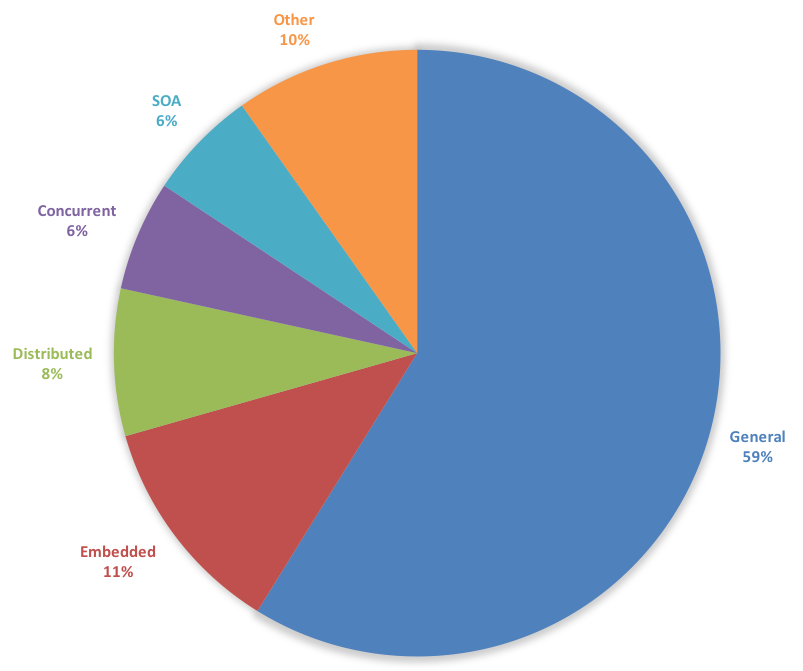
\includegraphics[width=0.6\textwidth]{Figures/litreview-adl-domains}
\caption{ADL Target Application Domain}
\label{figure:litreview-adl-domains}
\end{figure}

The analysis of the intended application domain of the languages can be found in \fref{figure:litreview-adl-domains}.  Interestingly very few of the languages were created for a specific business domain (e.g. financial analysis or industrial control systems) as over half the ADLs in the study do not explicitly target any business or technical application domain but are for general use.  There are a smaller number of ADLs specialised for embedded systems, distributed systems, highly concurrent systems and SOA, along with a number of individual ADLs for niche domains such as cyber-physical systems.

\begin{figure}
\centering
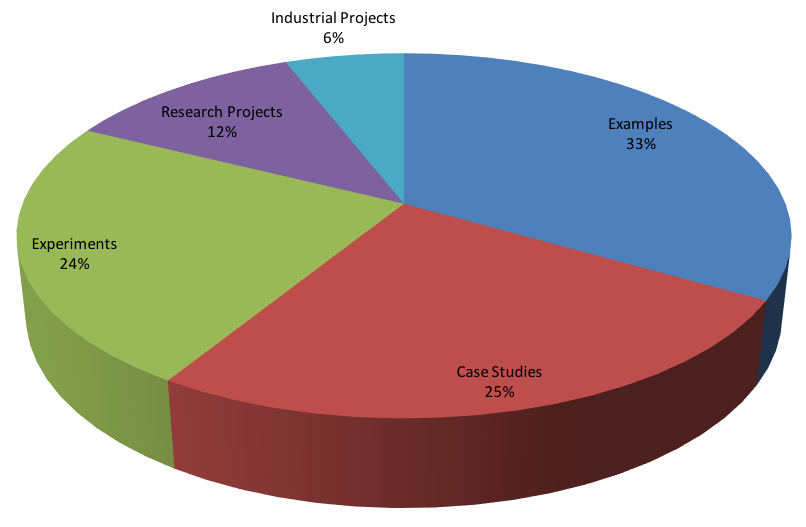
\includegraphics[width=0.6\textwidth]{Figures/litreview-adl-validation}
\caption{ADL Breadth of Application}
\label{figure:litreview-adl-validation}
\end{figure}

The analysis of the breadth of application of the languages can be found in \fref{figure:litreview-adl-validation}.  Unfortunately, as can be seen, less than 20\% of ADLs have been used beyond the case study level to perform significant research or industrial projects, suggesting a low degree of validation and practical experience with most of the languages.

The second area of interest to us were the \emph{architectural concepts} available in the different languages, to see if common industrial architectural concepts where in the languages or would need to be added.

The characteristics we analysed the ADLs for were the viewpoints that the ADL directly supports, the architectural concepts that they provide, whether they provide the ability to define behavioural semantics, whether they provide first class connectors and whether they provide first class architectural configuration constructs.  We chose to focus on these architectural concepts because of their wide use in the existing research literature and their general familiarity as concepts in industrial practice.

We were particularly interested in which viewpoints each ADL could support, as industrial architectural description nearly always needs a number of views to describe it, and the views supported provide a good insight into what the language can be used for.

None of the ADLs discuss a specific set of viewpoints that they define, so we analysed whether they provided effective support for the 6 viewpoints from \cite{rozanski2011-ssa2e} (which are Functional, Concurrency, Information, Development, Deployment and Operational).  We class a language has having first class connectors if the connector is defined separately to components and so is potentially reusable.  Similarly we consider architectural configuration to be a first class concept if it is described separately to the architectural elements and defines how they are combined, rather than being defined implicitly as part of the definition of the elements.

The complete data set for the architectural concepts available in each of the ADLs can be found in \tref{table:adl-concepts}.

The analysis of which viewpoints are supported by the different ADLs is presented in \fref{figure:litreview-adl-viewpoints}.

\begin{figure}
\centering
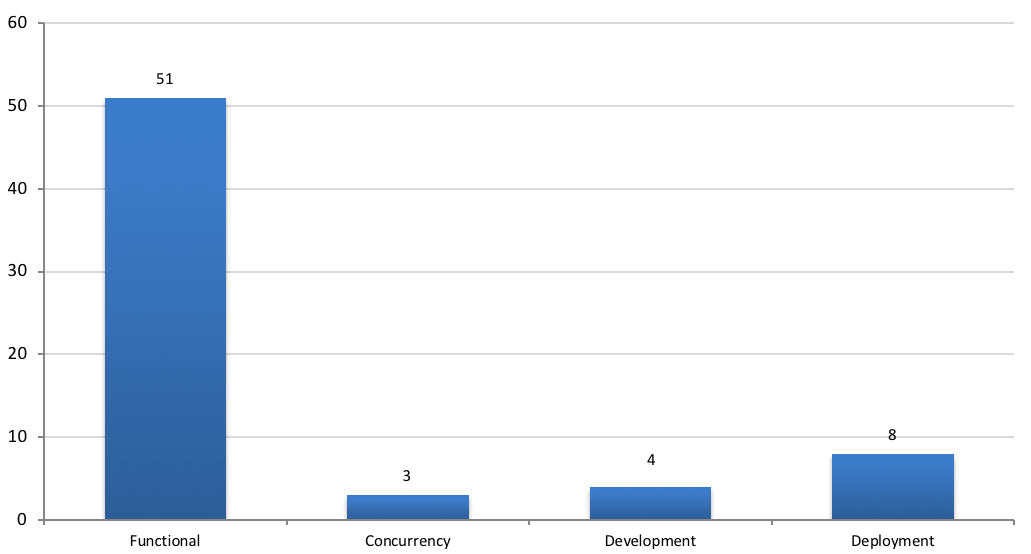
\includegraphics[width=0.75\textwidth]{Figures/litreview-adl-viewpoints}
\caption{Viewpoints Supported by ADLs}
\label{figure:litreview-adl-viewpoints}
\end{figure}

What is immediately evident from this analysis is that most ADLs only focus on the functional view of a system (i.e. its functional components and connectors and their organisation).  While clearly a key part of a system's architecture, most architects actually spend a lot of their effort working on other parts of an architecture (such as the deployment of the system).  So most of these ADLs are at best a partial solution to the problem of industrial architectural description.

\begin{figure}
\centering
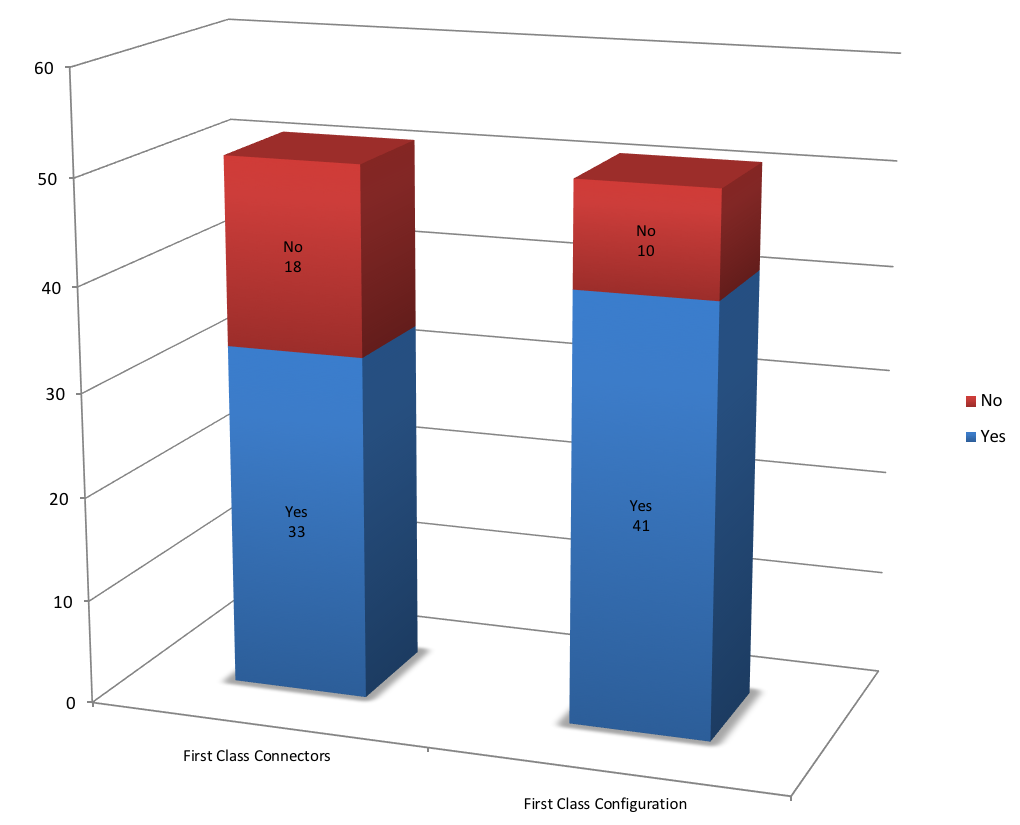
\includegraphics[width=0.75\textwidth]{Figures/litreview-adl-candc}
\caption{Connector and Configuration Support}
\label{figure:litreview-adl-candc}
\end{figure}

The analysis of the number of ADLs that provide support for first class connectors and architectural configuration as a first class concept is shown in \fref{figure:litreview-adl-candc}.

This analysis reveals a very positive result, as the clear majority of ADLs in the study provide some form of first class configuration, while less, but still nearly two thirds, provide support for first class connectors, which are both possible motivating factors for architects to use ADLs as existing informal and semi-formal notations tend not to support these concepts directly.

The third area of interest to us were the \emph{language mechanisms} available in the different languages, to assess the languages to see whether they could address common challenges (such as structuring and evolution) for large industrial architectural descriptions.

The attributes of the language that we analysed the literature for were as follows:
\begin{description} 
	\item[Structuring] - what mechanisms are available for structuring a large architectural description?
	\item[Evolution] - what mechanisms are provided to allow an architect to evolve an architectural description?  (Such as the ability to describe architectural variations, the ability to version all or parts of the description or support for dynamic architectures).
	\item[Qualities] - how provided or required architectural properties can be captured in the architectural description (e.g. properties, attributes, related models etc.).
	\item[Syntax] - what concrete syntaxes are available to capture architectural descriptions in the language?
	\item[Analysis] - how analysis of an architectural description could be supported using the language and any supporting technologies associated with it.
	\item[Tools] - what maturity are the tools that have been created to support the language? This can be "none", "prototype" (meaning an initial tool implementation applied to small problems), "research" (meaning a fully implemented tool applied to realistic problems by researchers), and "commercial" meaning that one or more tools have been implemented and used in an industrial context by people other than the tool's creators.
\end{description}

\begin{figure}
\centering
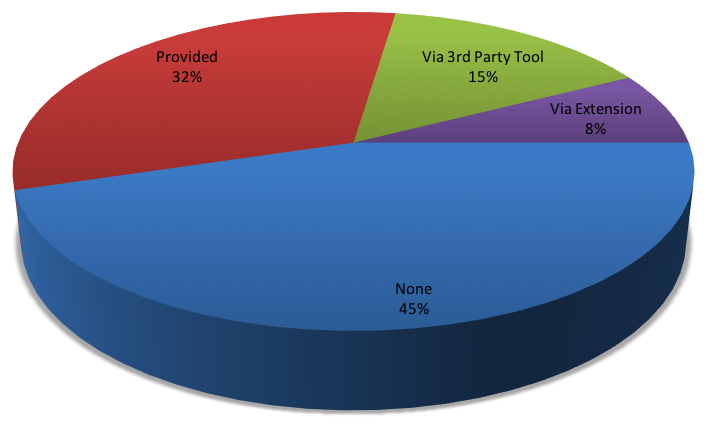
\includegraphics[width=0.6\textwidth]{Figures/litreview-adl-analysis}
\caption{ADL Support for Architectural Analysis}
\label{figure:litreview-adl-analysis}
\end{figure}

A common justification for using ADLs is the ability to perform automated analysis on the architectural description once it is represented using an ADL.  Therefore, we were interested to understand how many ADLs provided some sort of direct support for analysis of architectural descriptions.  

When we performed this analysis, we found that it was quite difficult because the analysis capabilities depend on support tools as much as the language and different ADLs provide quite different types of analysis capabilities.  To allow us to answer the question, we have defined four types of analysis capability:
\begin{description}
	\item [Provided] - where the ADL has specific support in the language to capture the data necessary to allow an automated tool to use it for analysis and explicit consideration has been given to making this possible.
	\item[Via Extension] - where the ADL has been designed such that its extension mechanisms could be used directly to support automated analysis via a tool.
	\item[Via 3rd Party Tool] - which means that the ADL provides some generic facilities that could allow a 3rd party tool to perform automated analysis, but where no explicit support for it is provided.
	\item[None] - where the language does not appear to be amenable to automated analysis.
\end{description}

This analysis is presented in \fref{figure:litreview-adl-analysis}.  As can be seen, less than half of the languages appear to provide realistic possibilities for automated analysis (and of course of those that do, many do not have working tools available for them).  We conclude therefore that automated analysis is only of interest in a subset of research groups working on ADLs.  A concern that we have with this situation is that an important motivator for adopting ADLs does not appear to be addressed in many of the ADLs that have been created.

\begin{figure}
\centering
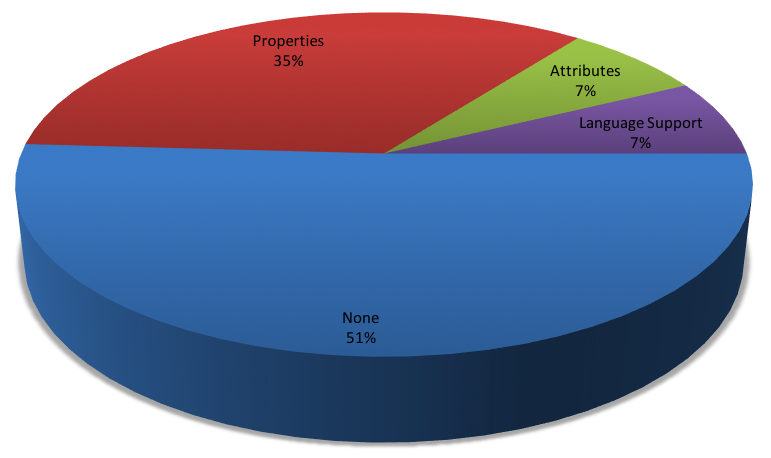
\includegraphics[width=0.6\textwidth]{Figures/litreview-adl-qualities}
\caption{ADL Support for Capturing System Qualities}
\label{figure:litreview-adl-qualities}
\end{figure}

A key goal of software architecture is to ensure that a system achieves the set of quality properties required for it to be successful.  This lead us to expect that ADLs would provide strong support for quality properties and we were interested in the types of mechanism used to represent them.  Having read the literature, we discovered that there were three broad levels of support for capturing quality properties in an architectural description:
\begin{description}
	\item[Properties] - where a generalised mechanism of (possibly typed) name/value pairs was available in the language and could be used to capture non-functional requirements and qualities but is not specifically provided for that purpose.
	\item[Attributes] - where specific pre-defined attributes relating to specific qualities (such as "transactions per second" for performance or "max connections" for scalability) can be captured within the language framework.
	\item[Language Support] - the case where languages provide a specific mechanism within the language for capturing quality requirements and capabilities (such as capturing security mechanisms and goals as first class language elements or providing a general purpose QoS or quality requirements sublanguage).
\end{description}

\fref{figure:litreview-adl-qualities} presents our analysis of this aspect of the capability of the ADLs.  It shows clearly that half of the languages provide no support for capturing system qualities, but that about a third (35\%) do have a generic properties mechanism which could be used to capture quality related information.  A much smaller number provide the ability to capture specific attributes (7\%) or have quality property features in their language (8\%).

\begin{figure}
\centering
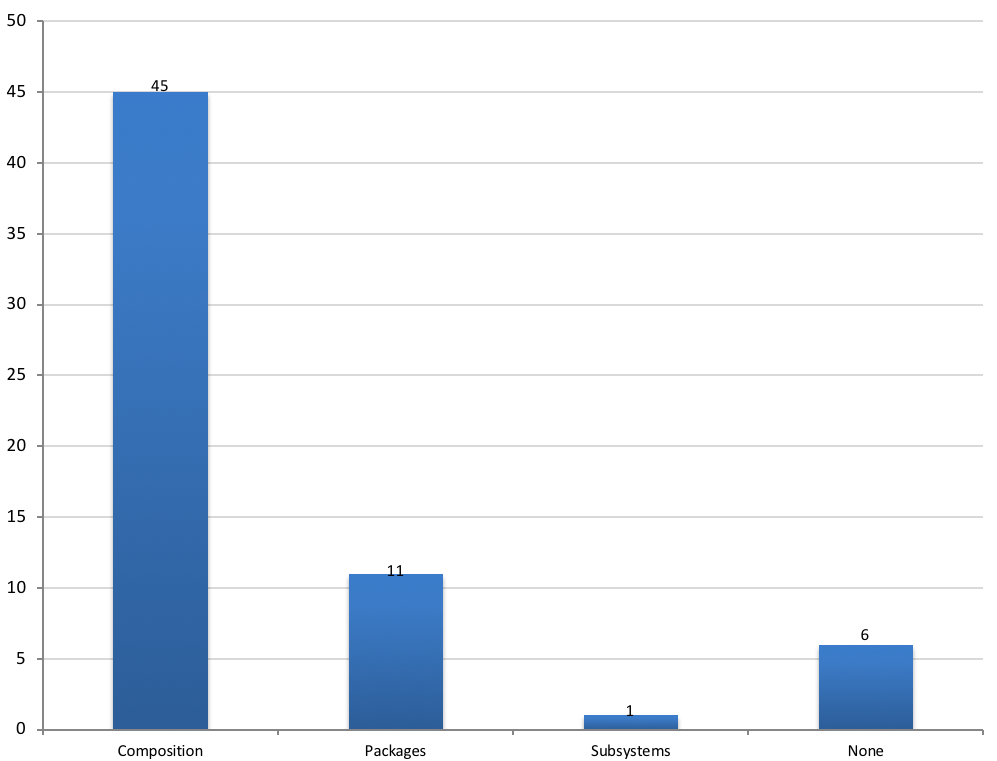
\includegraphics[width=0.75\textwidth]{Figures/litreview-adl-structuring}
\caption{Support for Structuring Architectural Descriptions}
\label{figure:litreview-adl-structuring}
\end{figure}

Many industrial systems are large, much larger than any case study or prototype experiment in the research domain.  A typical industrial system today can contain 500,000 to 1mm lines of code and dozens to hundreds of architectural elements.  Such systems cannot be described using languages that do not have effective structuring mechanisms to allow a system description to be broken down into smaller discrete parts.  This led us to investigate the mechanisms that each of the ADLs in the study provided for structuring the architectural description.  This analysis is shown in \fref{figure:litreview-adl-structuring}.

While a few of the ADLs (about 12\%) don't provide a structuring mechanism, most do, with nearly all of them offering \emph{composition} and a few offering \emph{packages} or \emph{subsystems} (in most cases in addition to composition - hence the total of values in the chart is larger than the number of ADLs in the study).
This is an interesting result, suggesting that most ADLs can be structured for large architectural descriptions, but that most of them utilise composition as the mechanism to achieve this, rather than providing a separate structuring mechanism like packages or subsystems.  This may imply restrictions in the flexibility of the structuring facilities available in those languages where only composition is available.

\begin{figure}
\centering
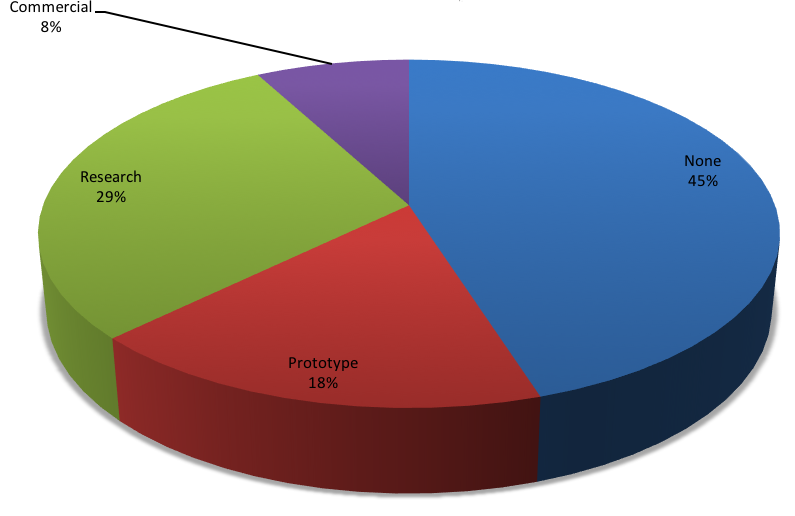
\includegraphics[width=0.6\textwidth]{Figures/litreview-adl-toolsupport}
\caption{Tool Support Available for ADLs}
\label{figure:litreview-adl-toolsupport}
\end{figure}

ADLs are often developed in conjunction with supporting tools to help architects to use them, which makes them more attractive for use on significant projects. \fref{figure:litreview-adl-toolsupport} presents our analysis of this feature of the ADLs in the study.

As can be seen, a very small percentage of the ADLs have commercially proven tools available to them, while about a third of them have tooling being used on research projects.  Nearly two thirds of the ADLs in our study provided no effective tool support.

\subsection{Answering the Survey's Research Questions}

\begin{description}
\item[ADL.RQ1] \emph{Which architectural viewpoints does each ADL support?}
All the ADLs in the study can represent functional views of the system and most of them only provide support for this view, but a small number of them allow deployment, concurrency or development views to be created too. Hence we conclude that the focus of most ADL research groups is how to represent the system's functional structure. This isn't surprising given how central a functional view is for most systems, but given the general acknowledgement of the importance of other viewpoints \cite{bachmann2011-documenting, brown2018-sad, kruchten1995-4plus1, rozanski2011-ssa2e} it does suggest that most of the existing ADLs will not be a complete solution to the problem of representing a software architecture.

\item[ADL.RQ2] \emph{Does the ADL provide structuring mechanisms for large ADs?}
Most ADLs in this study (45) provide the ability to structure a large architectural description by allowing composition of architectural elements (of course composition can also be used for other purposes, such as information hiding).   A smaller number provide specific mechanisms for structuring such as packages (11) and subsystems (1).  A few ADLs, surprisingly, do not appear to provide a structuring mechanism (6).  Some of the languages provide more than one mechanism that can be used to structure an AD (e.g. packages and composition) and this is why the numbers above sum to more than the number of ADLs in the study.\\
It is encouraging that most of the ADLs we surveyed provide at least basic facilities for structuring a large architectural description. This suggests that serious consideration has been given to the use of the ADL for realistic problems.  Those languages that don't allow structuring are presumably in an early stage of development or are not intended for industrial use.

\item[ADL.RQ3] \emph{Does the ADL support the analysis of an architecture?}
We found that about half of the ADLs (24 or 45\%) do not appear to allow a realistic option for automated analysis of architectural descriptions, which was something of a surprise to us.  Some of the languages do provide this though, with about 32\% of them providing direct support in the language, while 15\% allow this by providing mechanisms for 3rd party tools to embed information in the architectural description and 8\% allow for analysis by providing an extension mechanism that could allow analysis information to be added to an architectural description. \\
A clear motivation for capturing and maintaining an architectural description is the ability to gain useful and reliable automated analysis that can provide insight into the design that is otherwise difficult to obtain.  The fact that many ADLs being developed do not appear to provide analysis capabilities suggests that the problem of how to motivate others to use the language is often not part of the research process.

\item[ADL.RQ4] \emph{Can system qualities or quality requirements be captured in the ADL?}
Quality properties are central to the role and activities of the software architect and so we hoped for strong support for capturing qualities and quality requirements in the ADLs.  In fact, we found that more than half of the ADLs studied (28) do not appear to offer a facility to capture qualities and of those that do, most of them just provide a generic "properties" mechanism which can be used for a range of purposes including capturing qualities.  Only about 7\% of the languages provide quality property specific attributes in the language or include the ability to describe qualities as first class elements of the language.  This is a surprising situation, if the ADLs are expected to be used in an industrial setting.  Years of practical experience have taught us that achieving quality properties is a key objective of a software architect \cite{brown2018-sad, rozanski2011-ssa2e}, so we would have expected that supporting quality properties would have been an important requirement for an ADL.

\item[ADL.RQ5] \emph{Were prototype or production quality tools developed with the ADL?}
Given the importance of tool support in achieving adoption of new software technologies, we were surprised to find that 45\% of the ADLs in this survey do not appear to offer tool support that is ready for widespread transfer to industry and use.  29\% of the ADLs provide a tool that has been used for a research problem, and only 8\% of the ADLs have an associated tool that has been tested in an industrial context.\\
An important factor in applying ADLs on industrial projects is good tool support, preferably through extending tools that industry uses already.  In fact, we would go so far as to suggest that industrial adoption of any ADL without practical tool support is unlikely.

\item[ADL.RQ6] \emph{Has the ADL been applied to non-trivial problems outside the group of people who created it?}
Given the effort required to develop ADLs, we assume that most of them are intended for eventual technology transfer to industry.  Assuming so, the current degree of transfer out of the research groups is disappointing.  We found that 58\% of the ADLs have only been used by their creators, to create simple examples or experiments.  Another 26\% of the languages have only been used for case studies, again by their creators.  12\% appear to have been used for research projects, outside the creating group, while a mere 6\% of the languages have been applied in an industrial context. \\
It is our opinion that a technology can only be considered have had an impact when it is used by people other than its creators, and when considering the products of research groups, this means significant usage outside the originating research group and ideally in an industrial context.  Nearly all the ADLs we have surveyed fail this test, with less than 20\% of them having been used outside their originating group (based on the publications we could find).  It is possible that some of these ADLs have been used industrially but the case studies not published, however we feel that this is unlikely given the positive impact that publishing such case studies would have.  We believe that this finding in itself is cause for reflection within the ADL research community (as was the previous similar finding from a workshop some years ago \cite{woodshilliard2005-adlsinpractice}).
\end{description}



\section{Prioritisation of Architectural Effort}

TODO

\section{Application Energy Consumption Analysis} \label{sec:litreviewenergy}

TODO
